\subsection{Workshop: Workshop on Deep Learning and Inverse Problems}

\subsubsection{Uncertainty Quantification in Deep MRI
Reconstruction \cite{edupuganti2020uncertainty}}

Presented by \textit{Vineet Edupuganti} \\

{\bf Motivation:} accelerated MRI reconstruction is unreliable, especially when generative models are applied. Need to estimate uncertainty of a reconstruction model to help radiologist to avoid mistakes. \\

{\bf Background:} most of existing approaches (Deep Ensembles \cite{Lakshminarayanan17}, VAE sampling \cite{corr/abs-2007-08128}) for epistemic uncertainty estimation leverage one or another form of the Monte Carlo sampling: several samples are utilized to compute statistics, which are then represented as results. One example of this approach is to sample from VAE and compute variance of results. However, it is impossible to compute bias without ground truth image using this method. \\

{\bf Method:} authors propose to utilize  Stein’s Unbiased Risk Estimator
(SURE) \cite{doi:10.1080/01621459.2018.1429276} to compute bias-free uncertainty estimation without reference image. For that, the following derivation is performed.

Given the ground truth image $x_0$, the zero-filled image can
be written as 

\begin{equation}
    x_{zf} = x_0 + v
\end{equation} 

where $v$ is noise. Now considering reconstruction $\hat{x}$ with
dimension $n$, one can expand test MSE as 

\begin{equation}
    \mathbb{E}|| \hat{x} - x_0 ||^2 = \mathbb{E} || x_0 - x_{zf} + x_{zf} - \hat{x} ||^2 = -n \sigma^2  + \mathbb{E} || x_{zf} - \hat{x} ||^2 + 2Cov(x_{zf}, \hat{x})
    \label{eq:sure-one}
\end{equation} 

Since $x0$ is not present in \ref{eq:sure-one}, we see that SURE serves as a surrogate for MSE even when the ground truth is unknown. 
A key assumption behind SURE is that the noise process v that relates the zero-filled image to the ground truth is normal, namely $v \sim N(0, \sigma^2
I)$. 
With this assumption SURE is formulated as follows 

\begin{equation}
    SURE = -n \sigma^2 || \hat{x} - x_zf ||^2 + \sigma^2 tr(\partial \hat{x} / \partial x_zf)
\end{equation}

\textbf{Important note:} previous assumption may not hold in practice. 

Authors show that when error in the output reconstruction is not large, and as a result $\sigma^2$ can be estimated as 

\begin{equation}
    \sigma^2 = || \hat{x} - x_{zf} ||^2  / n
\end{equation} 

This assumption allows to formulate SURE as follows 

\begin{equation}
    SURE = \sigma^2 tr(\partial \hat{x} / \partial x_zf)
\end{equation} 

\textbf{Important note:} this assumption on only holds for low acceleration rates and artefact-free reconstruction models. 
Since this method is developed for evaluation of potentially artefact-prone models, this assumption looks quite strong. \\

Further investigations are targeted on acceleration of computations of trace of the end-to-end network Jacobian, which otherwise can be problematic. 
Authors also approach the problem of the requirement for MRI noise to follow standard normal distribution. \\

{\bf Results and takeaways:} the main contribution of this work is to apply SURE to the uncertainty estimation task in the domain of medical imaging, which has not been done before. 
An example of high correlation between estimated SURE values are computed MSE error is illustrated on figure \ref{fig:sure-result}.

\begin{figure}[h!]
    \centering
    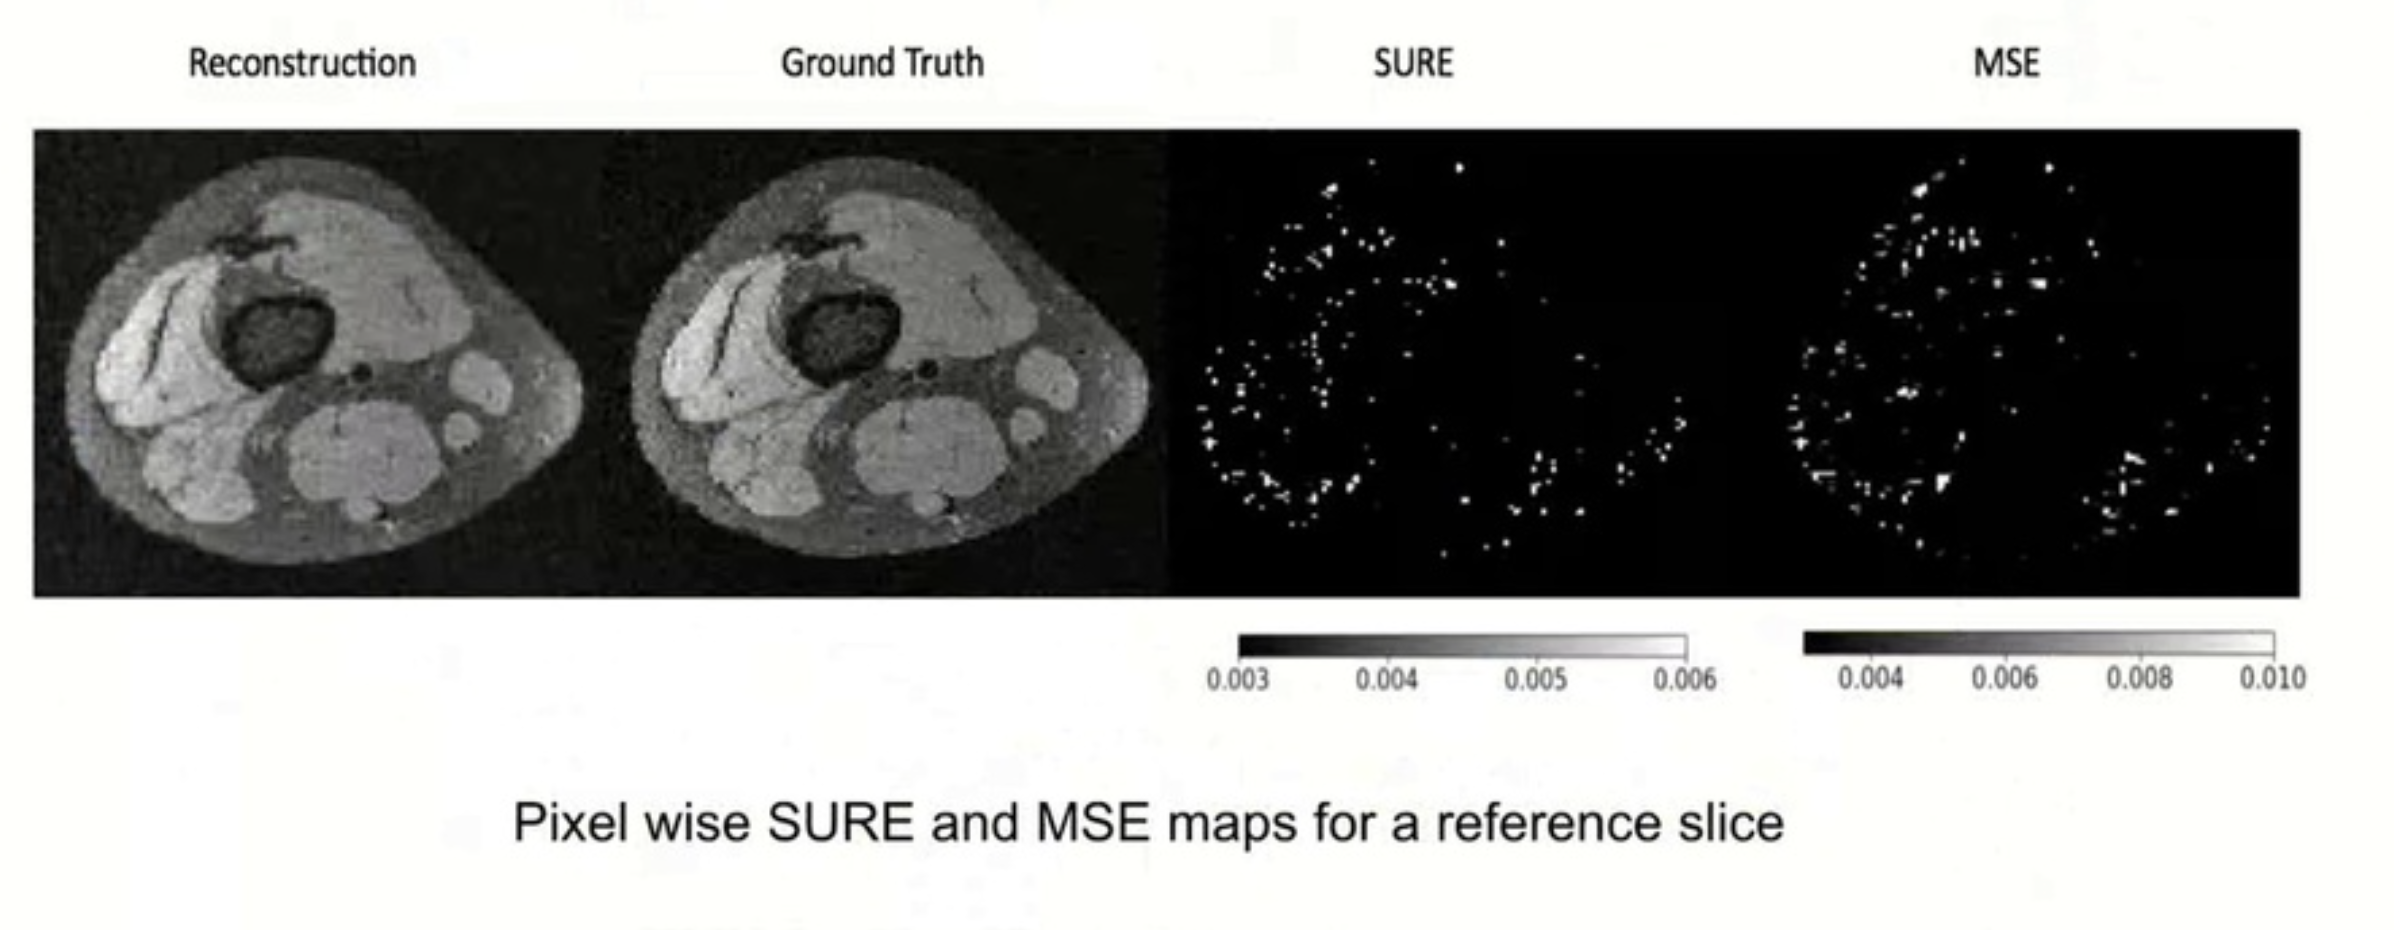
\includegraphics[scale=0.4]{neurips-2020/images/Screenshot 2020-12-12 at 17.26.28.png}
    \label{fig:sure-result}
\end{figure}





\subsubsection{ \cite{}}

Presented by \textit{} \\
